FreEBS is a virtual block device backed by replication and log-structured
virtual disks for high reliability and availability. For all intents and 
purposes, the FreEBS storage system appears to the kernel as a normal block
device and thus reads and writes are issued to FreEBS without knowledge of 
its internals. The architecture of FreEBS is depicted in 
Figure~\ref{fig:architecture}. As we observe, the most important component in
the system is the \emph{driver}, which is a mountable kernel module that 
interfaces between the OS and the rest of the system. It accepts normal 
block device commands and forwards the requests appropriately to the 
\emph{replicas}. Our current configuration uses three replicas, but our 
design is flexible enough that we can arbitrarily add more if necessary. We 
discuss replication in more detail in Section~\ref{sec:replication}.
 
Replicas are essentially server machines that communicate with each other 
and the driver across the network using a custom TCP protocol. Each replica 
runs a userspace process called \texttt{sdaemon} that is in 
charge of propagating write requests and synchronizing replicas. It is also
responsible for interfacing with its private copy of the underlying storage 
that actually holds the device data, \emph{Log Structured Virtual Disk}
(LSVD). LSVD is backed by a file on the server file system that uses a 
dynamically growing file format. It provides checkpointing and versioning 
for high data integrity. A more in-depth discussion about LSVD is in 
Section~\ref{sec:lsvd}.

\begin{figure}[h]
    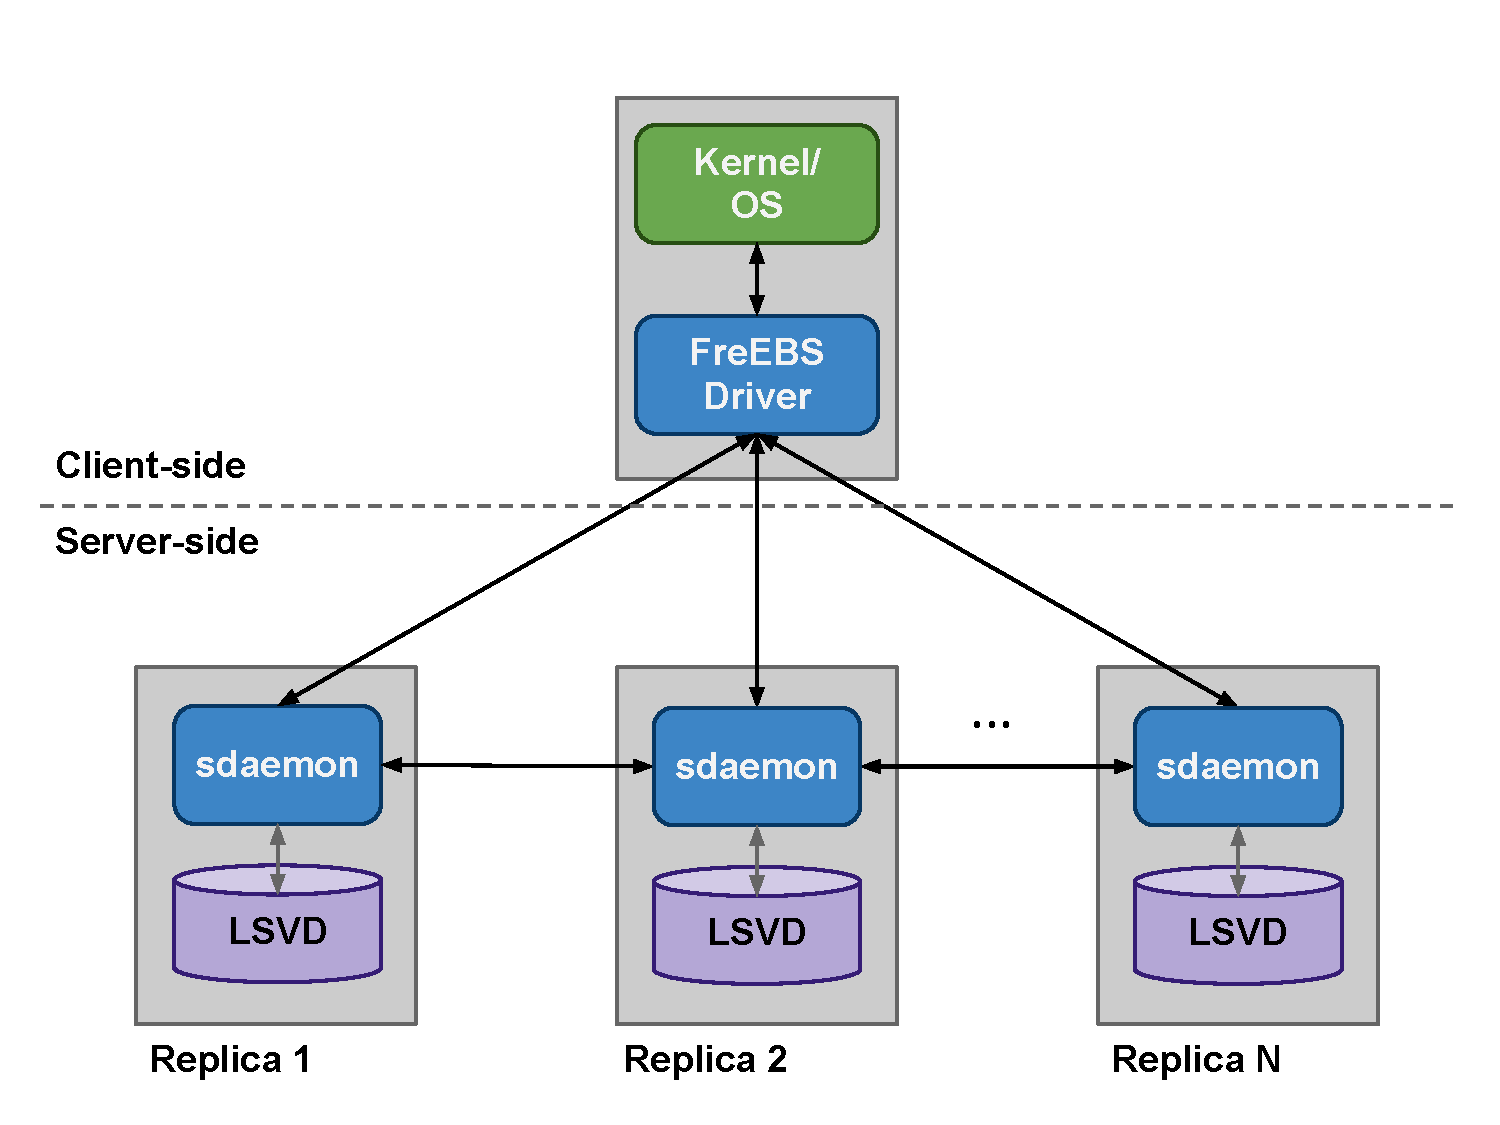
\includegraphics[width=0.45\textwidth]{./figures/systemarch.pdf}    
    \caption{The system architecture for FreEBS. A driver on the client 
            machine communicates with processes on the replicas on server 
            machines to read and write data.}
    \label{fig:architecture}
\end{figure}


